\chapter{Scaling bitcoin}

There is no secret that the Bitcoin blockchain will not be able to scale on its own. When Nakamoto first published the whitepaper on the cryptographic mailing list his first response was in fact that such a solution won't scale very well~\cite{donald:scale}. 

Andreas Antonopoulos has drawn similarities between the scaling of bitcoin with the scaling of the internet:

\begin{displayquote}
	"Bitcoin is failing to scale. If we’re really lucky, bitcoin will continue to fail to scale gracefully for 25 years, just like the internet."~\cite{antonopoulos:the:internet:of:money}
\end{displayquote}

This quote is accurate as Usenet used a \textit{Store-and-forward} method for content to reach every server in the network. \textit{Store-and-forward} does not scale very well and is somewhat similar to the base \gls{bitcoin} protocol. The internet moved away from \textit{Store-and-forward} to more direct routing and Bitcoin is too, allowing transactions to happen off-chain.

In this chapter the various scaling alternatives will be discussed.

\section{Block Size limit}

In 2010 Nakamoto reduced the block size limit from 32 to 1 Megabyte with two commits. The first commit introduces the new \texttt{BLOCK\_SIZE\_LIMIT} constant~\cite{nakamoto:commit:1} and the other commit enforcing the blocks to be under the limit~\cite{nakamoto:commit:2}. Nakamoto did not give any explanation as to the reason of this limit. As there was only a few transactions per block at this time a limit reduced the worst case scenario for a \textit{Denial-of-Service} attack where blocks are filled with dummy transactions. 

Increasing the amount of transactions would also increase the imposing cost for the ecosystem by forms of bandwidth, processing and storage - reducing the speed by which the blocks propagate through the network. By imposing a block limit the cost of operating a node would be kept low allowing more peers to be able to participate in the network. 

% would come at an increased cost for the ecosystem (bandwidth, processing, and storage for relay nodes, as well as an impact on propagation speed of blocks on the network

With a limit on 1 Megabyte; Bitcoin is capable of ~10 transactions per second or 350.000 per day. This in contrast with a traditional payment processor such as visa who have capacity 65.000+ transactions per second\cite{visa:fact:sheet}. In it's current form Bitcoin does not have close to enough capacity as a payment processor for a significant fraction of the global economy.

\section{Increasing block size limit}

There has been many proposals to increase the block size. Including a handful of \gls{bip}s:

\begin{itemize}
	
	\item \textbf{BIP 100} allows the miner to vote on the block limit by encoding a proposed value in the coinbase unlocking script. A 75\% supermajority may increase the block size limit every 2016 blocks. Each period change is limited to only increase by 5\% from the previous period.~\cite{bip:0100:dynamic:block:size}
	
	\item \textbf{BIP 101} proposes an immediate increase to 8 megabyte blocks and continue to double every second year. In the two year periods the size would increase at a linear pace based on the block timestamp.~\cite{bip:0101:increase:block:size}
	
	\item \textbf{BIP 102} is a simple one time increase to 2 megabytes. The BIP would be triggered if 95\% of the latest blocks signaled support for the upgrade.~\cite{bip:0102:increase:2mb}
	
	\item \textbf{BIP 103} aims to increase the block size in accordance with the technology. In practice however it increases the block size with 4.4\% every ~97 day, 17.7\% annually.~\cite{bip:0103:increase:with:technology}
\end{itemize}

Most of these \gls{bip}s are implemented as a hard forks. Older nodes would regard the bigger blocks as being over the limit and thus invalid.
If poorly executed, without a great majority upgrading the software in time, the network would be forked into two networks with diverging transaction histories. 

% need better name for community worker
\subsection{Contentious Hard Forks}

No proposal to increase the block size has yet received enough support to be activated. This has caused some controversy among community members and multiple have attempted to increase the limit by force. 

One of the earliest attempts to increase the block size was when node Bitcoin XT implemented BIP 101 mentioned above. It failed to reach the miner consensus it required to activate. The BIP 101 was then removed and replaced by a 2 megabyte block limit which forked bitcoin into an additional network - Bitcoin Classic. Mike Hearn, co-creator of Bitcoin XT along with Gavin Andersen, has made his intention clear arguing that the block size must increase for bitcoin to reach any adoption beyond a fringe niche~\cite{hearn:classic}. 

\begin{figure}[!htb]
	\hspace*{-0.7cm} 
	\centering
	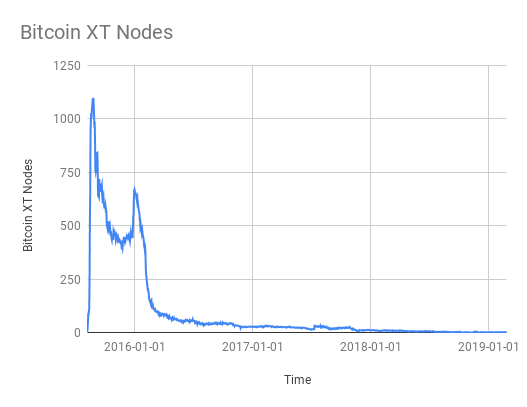
\includegraphics[width=8cm]{external/Bitcoin_XT_Nodes.png}
	\caption{\textit{Historic Bitcoin XT node count. As of 2019-02-25 only three nodes are still active. Data retrieved from coin.dance~\cite{coin:dance}.}}
	\label{fig:xt_nodes}
	\hspace*{2mm} 	
\end{figure}

As figure \ref{fig:xt_nodes} attests, bitcoin XT and classic failed to receive support and is now dead.

\subsection{The Bitcoin Cash saga}

The failures of Bitcoin Classic were just the beginning of the scaling debate. The proposal of Segregated Witness~\cite{bip:0141:segwit} was met with strong opposition as it was considered an overtly complicated and risky upgrade when the block limit could simply be increased. 

Segregated Witness is in a way an increase in block space as it moves the unlocking script(witness) from the transaction to its own structure. Since each transaction takes up less space, more transactions fit in each block. The upgrade also addresses malleability, which many off-chain solutions require, and aligns economics incentives with resource costs~\cite{antonopoulos:segregated:witness:align:economic:incentives}. Although its possible to implement the Lightning Network without a malleability fix, it increases its viability~\cite{song:lightning:malleability}.

The malleability fix also addresses covert \texttt{ASICBOOST} or \texttt{ANTBLEED}. Covert \texttt{ASICBOOST} utilizes that part of \texttt{SHA256} may be pre-calculated if the last 16 bits remain the same. The last 16 bytes in the bitcoin header include the last 4 bytes of the Merkle root. By finding two Merkle Roots with the same last 4 bytes, allowing for less computation in finding \gls{hash}es. To find a matching pair of roots, many roots must on average be tried. The space of viable roots is reduces if the transaction witness isn't malleable~\cite{song:asicboost} as the witness can't be manipulated to change the transaction and thus the Merkle root. Gregory Maxwell alluded that \texttt{ASICBOOST} had in fact been implemented in ASIC chips and proposed a fix~\cite{maxwell:asicboost:fix}. Bitmain, the largest chip manufacture, made a statement two days later addressing Maxwell's accusation~\cite{bitmain:response}. There is no way of ultimately proving if covert \texttt{ASICBOOST} was ever used\footnote{In further conversation with Bitmain representative Nishant Sharma at their headquarters in Beijing in December 2017 he stated that they would never use \texttt{ASICBOOST} of moral reasons. \texttt{ASICBOOST} was not longer viable on \gls{bitcoin} at that time, but was on Bitcoin cash and other currencies. He also stated that Bitmain had been in negotiation to buy the patent from Timo Hanke and Sergio Demian Lerner and had thus filed a patent for \texttt{ASICBOOST} with the Chinese government. The deal ultimately didn't fell through, and while this information is hearsay at best, the patent sparked many rumors at the time and drove opposition and is one reason for the eventual split.}. 

When~BIP148~\cite{bip:148:uasf:segwit}, a \textit{user-activated-soft-fork} scheduled for 22 August 2017 to activate Segregated Witness, was getting traction among \gls{node}s, the opposing party(including aforementioned Bitmain) decided to hard fork bitcoin into two by raising the block size limit. The hard fork took place on the first day of August 2017 and created Bitcoin Cash.

Bitcoin Cash received significant economic support initially, although significantly below the original chain.

\begin{figure}[!htb]
	\hspace*{-0.7cm} 
	\centering
	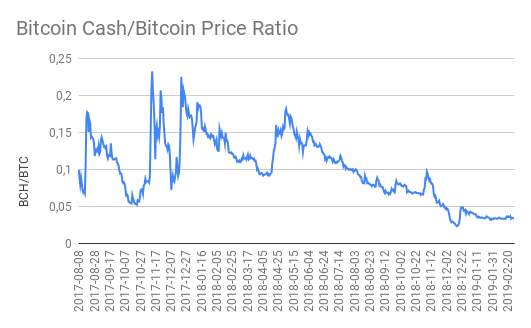
\includegraphics[width=8cm]{images/Bitcoin_Cash_Bitcoin_Price_Ratio.png}
	\caption{\textit{Historic Bitcoin Cash/Bitcoin price ratio. Data retrieved from Yahoo Finance.}}
	\label{fig:bch_btc}
	\hspace*{2mm} 	
\end{figure}

Although support for Bitcoin Cash has dwindled over the following years, it set a precedence of how forks may be utilized. It also showed that support from miners is not necessary. During the second half of 2017 many more forks happened similarly to bitcoin cash.

\subsection{The SegWit2x Compromise}

Most forks are insignificant. However SegWit2x carry some historical weight. SegWit2x was originally a compromise known as the Hong Kong Agreement reached in Hong Kong in February 2016 between many industry representatives and members of the development community~\cite{hong:kong:agreement}. The agreement was somewhat ambiguous leading to fall out and a subsequent New York Agreement were reached at the Consensus conference in May 2017~\cite{new:york:agreement}. Notable absent from the latter agreement were the whole Core development team leading to the \texttt{UASF} and Bitcoin cash fork. Many actors still viewed the New York Agreement as valid after the split and many supported a hard fork to 2MB block limit on the main Bitcoin chain in late 2017. The fork was ultimately called off and only a few rogue actors followed through with it. A critical bug in the software led to the forked chain to halt in it's infancy. 

\section{Removing or reducing decentralization}

Many other cryptocurrency systems, which are seen as competing, have reduced decentralization in order to increase throughput. Some may not even be considered \textit{peer-to-peer} but instead rely on a traditional \textit{client-server} architecture which current financial systems are already using. These system easily scale. Most however use some sort of combination of increased block limit and/or some level of trusted \gls{node}s akin to \textit{oracles}.  

\section{Sidechains}

One proposal involve multiple chains where one could peg bitcoin to an alternate, less secure, chain. Multiple transactions could then take place on the alternate chain and then released back on the main chain. The alternate chains could regularly be thrown away and replaced, removing much of the storage burden of the network.~\cite{blockstream:sidechain}

\section{Off-chain scaling}

Off-chain solutions, like the \gls{Lightning Network}, utilize the contractual nature of transaction. Schemes of transactions can be implemented such as that an obligation, in form of a transaction, may be held privately without broadcasting it. The obligation may then be changed multiple times without the rest of the network knowing and only in worst case, require to broadcast the transaction. 

Most schemes involve payment channels, where two parties locks in funds between each other and then the balance between them can be updated without using the blockchain. Multiple channels may be aggregated together into a network. Consider a channel between Alice and Bob and a channel between Bob and Carol. If Alice wish to pay Carol, she may update her channel with Bob if and only if Bob updates his channel with Carol.  

Payment channel networks may be constructed in many different ways, a few distinct proposals has been suggested. Decker and Wattenhofer suggested a scheme with Duplex micropayment channels~\cite{decker:wattenhofer:duplex}. The \gls{Lightning Network} is further discussed in the following chapter. Recently a new scheme was published, the eltoo protocol, which may be integrated into the Lightning Network stack~\cite{decker:russell:Osuntokun:eltoo}.   

\section{Rationale for small blocks}

\gls{bitcoin}s advantage does not lie in its ability to scale. In fact, centralized solutions can trivially outperform Bitcoin many times over with regard to cost, speed and reliability. Its strength lie in transparency, immutability and that it require no trust in any other party at all. These characteristics are both unique and valuable. Solutions to scale the network ought to not compromise the fundamental properties making it worth to scale in the first place. Therefor the cost of participation must remain low, which require that the cost of validating blocks must remain low and thus require small blocks.
